\documentclass[11pt]{article}
\usepackage[margin=1in]{geometry}
\usepackage{graphicx,longtable,array}

\title{A proteome-wide fixed-difference structural atlas distinguishes mpox clade Ib from the 2022 clade IIb outbreak strain}
\author{Computational analysis, open public data (science-program project 7)}
\date{September 23, 2026}
\begin{document}
\maketitle
\begin{abstract}
\textbf{Background.} Mpox clade Ib emerged in the Democratic Republic of the Congo in 2023 and,
like the 2022 clade IIb lineage B.1 outbreak strain, sustains human-to-human transmission, but with
a distinct epidemiological pattern. Which protein-level differences separate the two outbreak clades
had not been mapped proteome-wide. \textbf{Methods.} From frozen Pathoplexus/LAPIS aggregates
(dataVersion 1790097064; open INSDC data) we extracted every fixed amino-acid difference between
clade Ib (n=377 complete genomes, completeness $\geq$0.95) and clade IIb B.1 (n=3578), requiring
$\geq$0.95 within-clade frequency at covered positions, polarized each difference with a clade Ia
outgroup (n=511), classified every differing protein (surface/immune/replication-assembly/unknown)
under locked rules, and mapped prioritized changes onto ESMFold models with a pLDDT $\geq$ 70
confidence gate. Success gates and thresholds were locked in writing before outcomes were examined;
both positive controls passed (published complement-control-protein loss recovered in 25/25 raw Ib
genomes; published APOBEC3 signature reproduced in IIb B.1). \textbf{Results.} We identify 291
fixed protein-level differences (264 substitutions, 27 deletions). Only 38 are derived in clade Ib;
the remainder are clade-I background on which IIb B.1 is the derived state. Ib-derived changes are
significantly concentrated on virion-surface proteins (20/38, 52.6\% vs 23.3\% of background;
one-sided hypergeometric $p=3\times10^{-4}$). The largest is an in-frame 13-residue deletion
(R134--V146) in OPG164 (A36R IEV transmembrane phosphoprotein), the actin-tail protein that drives
cell-to-cell spread, deleting a low-complexity cytoplasmic tail segment immediately downstream of
the phosphorylation region. Further Ib-derived surface changes hit the immunodominant B22R family
protein (A475V, E1057D), hemagglutinin (T239I), and IMV proteins A14, E8 and J1. Both clades show
indistinguishable APOBEC3-type fractions among recent substitutions (32.9\% vs 33.0\%), indicating
equivalent sustained human transmission pressure; the clades differ in what changed, not in the
mutational process. \textbf{Conclusions.} Clade Ib's distinguishing evolution is surface-focused,
headlined by a 13-aa deletion in the virus's actin-based spread machinery and changes to the
immunodominant B22R family protein --- a plausible mechanistic basis for its distinct spread
pattern, and a prioritized target list for experimental follow-up.
\end{abstract}

\section{Introduction}
Monkeypox virus (MPXV) is a double-stranded DNA orthopoxvirus with a genome of roughly 197 kb
encoding $\sim$180--200 proteins. Two major clades circulate in humans: clade I (Central Africa,
historically higher virulence) and clade II (West Africa). In 2022, clade IIb lineage B.1 caused a
multi-country outbreak driven by sustained human-to-human transmission, prompting WHO to declare a
Public Health Emergency of International Concern. In 2023--2024, a new clade I sublineage, clade Ib,
emerged in eastern Democratic Republic of the Congo and spread regionally and internationally,
again via sustained human-to-human transmission but with a different epidemiological profile,
triggering a second PHEIC in August 2024.

Prior genomic comparisons established that clade Ib carries a novel $\sim$1.1 kb deletion removing
the complement control protein (CCP) and clade-specific changes in the B22R receptor-binding protein
(bioRxiv 2024, doi:10.1101/2024.09.24.614696), that APOBEC3-driven editing marks sustained human
transmission in both clades, and that single mutations can remodel entry-fusion-complex interfaces
(Molecules 2026, doi:10.3390/molecules31091466). What has been missing is a systematic,
proteome-wide account of \emph{which} protein-level differences are fixed between clade Ib and the
2022 IIb B.1 outbreak strain, which of them are new in Ib rather than clade-I heritage, and whether
their distribution across protein classes plausibly bears on the different spread patterns.

Here we build that atlas. Every step runs on open public data with frozen inputs, locked success
gates, positive-control validation before any novel claim, and honest accounting of confidence.

\section{Methods}
\subsection{Data}
All sequence data come from the Pathoplexus LAPIS instance for mpox
(\texttt{https://lapis.pathoplexus.org/mpox}), which ingests open INSDC genomes and aligns them against
reference NC\_063383.1 (clade IIb, 2018). We froze dataVersion 1790097064 on 2026-09-23. Three
quality-controlled sets were defined by aggregated queries (completeness $\geq$ 0.95): clade Ib
(n=377), clade IIb lineage B.1 (n=3578), and clade Ia as outgroup (n=511). Aggregated amino-acid
mutation tables (counts, coverage, proportion per mutation vs the reference) were pulled for all
three sets; nucleotide mutation tables for Ib and IIb B.1. Reference annotations: NC\_063383.1
(179 CDS, gene table parsed programmatically) and NC\_003310.1 (clade Ia, Zaire-96-I-16). An
independent validation set of 45 complete raw genomes (25 Ib, 10 Ia, 10 IIb B.1) was fetched from
NCBI efetch. Every input file is checksummed (SHA256SUMS.txt) and every query URL recorded
(data/MANIFEST.md).

\subsection{Fixed differences}
For each (gene, position) we assigned each clade set its dominant residue (highest-proportion state
in the aggregated mutation table; positions absent from a set's table were assigned the reference
residue, valid because LAPIS reports mutations with proportion $\geq$ 0.05). A \emph{fixed
difference} requires: dominant residues differing between Ib and IIb B.1; dominant proportion
$\geq$ 0.95 in both sets; positional coverage $\geq$ 100 (Ib) and $\geq$ 1500 (IIb B.1) sequences.
Deletions (gap residues) count as differences. These thresholds were locked before inspecting
outcomes.

\subsection{Polarization}
Each fixed difference was polarized against the clade Ia consensus under the same frequency and
coverage rules: \emph{Ib-derived} when Ia matches IIb B.1; \emph{IIb-derived} (clade-I background in
Ib) when Ia matches Ib; \emph{three-way} when all differ.

\subsection{Classification}
Every differing protein was classified as surface-exposed, immune, replication-assembly, or unknown
by a locked keyword rule order over the reference annotation product string, with three curated
overrides (OPG123 NPH-I, OPG125 rifampicin-resistance locus, OPG098 VP8/L4R core protein; all
replication-assembly). The rule that fired is recorded per row. Enrichment was tested with the
one-sided hypergeometric tail.

\subsection{Structures}
AlphaFold DB does not cover the current MPXV UniProt accessions (checked programmatically:
0/110 mapped genes), so we folded selected Ib-derived target proteins ($\leq$400 aa) with the public
ESMFold API, plus reference versions of the two deletion proteins. Per locked gate G3, structural
statements are made only where per-residue pLDDT $\geq$ 70; below-cutoff positions are reported as
sequence-level findings. No large-scale structure prediction was attempted.

\subsection{Positive controls (run before novel claims)}
\emph{G2a.} The published CCP (OPG032) loss in clade Ib must be recovered from raw genomes: we
probed the 651-nt clade-Ia CCP gene with three 60-mers (plus a tolerant 20-mer check) across the 45
raw genomes. \emph{G2b.} The published APOBEC3 enrichment must be reproduced in IIb B.1:
substitutions in TC$\rightarrow$TT or GA$\rightarrow$AA contexts vs a uniform null over the
reference sequence.

\subsection{APOBEC3 comparison}
To compare \emph{recent} mutational processes fairly between clades, we extracted terminal/internal
branch nucleotide substitutions per clade from the Nextstrain all-clades mpox build
(data.nextstrain.org, updated 2026-09-16; 803 leaves) and computed APOBEC3-type fractions against
the same reference context.

\subsection{Reproducibility}
The full pipeline is four scripts; re-running code/01 from the frozen inputs regenerates the
fixed-difference table byte-identically (verified). All code, manifests and tables are in the
project repository.

\section{Results}
\subsection{291 fixed protein-level differences separate the outbreak clades}
We find 291 fixed differences between clade Ib and clade IIb B.1 across 119 of 179 reference CDS:
264 substitutions and 27 deletions (Table A1). Per-position coverage requirements were met
everywhere reported; the Ib set contributes $\geq$100 observed sequences at every called position.

\subsection{Only 38 differences are new in clade Ib --- and they cluster on the virion surface}
Polarization against clade Ia assigns 38 differences as Ib-derived, 250 as clade-I background on
which IIb B.1 carries the derived state, and 3 as outgroup-uncertain. Ib-derived changes are
significantly enriched on surface-exposed virion proteins: 20/38 (52.6\%) vs 59/253 (23.3\%) among
background differences (one-sided hypergeometric $p=3\times10^{-4}$; Figure 2). Immune-modulatory
and replication-assembly classes are correspondingly \emph{depleted} among Ib-derived changes.

\subsection{Headline structural change: a 13-residue deletion in the actin-spread protein OPG164/A36R}
The single largest Ib-derived change is an in-frame deletion of residues R134--V146 of OPG164, the
IEV transmembrane phosphoprotein orthologous to vaccinia A36R. In vaccinia, A36R's cytoplasmic tail
is phosphorylated (Tyr112/Tyr132 region) and recruits Nck/Grb2 adaptors and NPF-motif interactors to
drive actin-based motility and cell-to-cell spread (Frischknecht et al., Nature 1999; Humphries et
al., Nat Microbiol 2016). The deleted segment lies immediately downstream of that phosphorylation
region. ESMFold models of both variants place the segment in a low-complexity, low-confidence tail
(mean pLDDT $\sim$40 over residues 134--146; Figure 4); per gate G3 we therefore make the
sequence-level claim (an in-frame 13-aa deletion fixed at $>$0.95 frequency across 377 Ib genomes)
and note that the affected region is a signaling-motif-bearing disordered tail, not a folded domain.
A 2-aa N-terminal deletion (V16--H17) is likewise fixed in OPG045, a caspase-9-inhibitor family
immune protein.

\subsection{The immunodominant B22R family protein and other surface antigens carry Ib-derived changes}
OPG210 (B22R family protein, 1881 aa) carries two fixed Ib-derived substitutions (A475V, E1057D).
Poxviral B22-family proteins inhibit T-cell activation and increase virulence (PLOS Pathog 2014,
doi:10.1371/journal.ppat.1004123), and B22R is a dominant serological target in mpox. Additional
Ib-derived surface changes: hemagglutinin OPG185 T239I, IMV membrane proteins A14 (OPG140 P39H),
E8 (OPG070 Y12H), J1 (OPG100 R134H), crescent-membrane protein OPG096 L75P, and chemokine-binding
protein OPG170 V96I.

\subsection{Replication machinery changes are mostly clade-I background}
Ib-derived replication-assembly changes are few and conservative (DNA helicase OPG145 P76Q, rpo132
OPG151 R273Q, core protein P4a OPG136 M740I, late transcription factor VLTF-2 OPG126 A26S, RNA
polymerase 30 kDa OPG066 K140N/L222I, rifampicin-resistance protein OPG125 T493M).

\subsection{Both clades show the same APOBEC3 signature of sustained human transmission}
Among recent branch substitutions in the Nextstrain all-clades build, APOBEC3-type contexts
(TC$\rightarrow$TT/GA$\rightarrow$AA) account for 32.9\% in clade Ib (331 substitutions) and 33.0\%
in clade IIb (1570), both $\sim$16-fold above the 2.1\% uniform null (Figure 3). The positive
control on IIb B.1 LAPIS data independently reproduced the enrichment (35.3\% vs 2.1\%; G2b pass).
Thus both clades have been under comparable sustained human-to-human transmission pressure; their
biological differences are encoded in the fixed protein changes, not the mutational engine.

\subsection{Positive-control caveat discovered and preserved}
The CCP probe confirmed deletion in 25/25 Ib and 10/10 IIb B.1 raw genomes and presence in canonical
Ia references --- but 4/10 recent Ia genomes (2024 DRC, FV537349--52) also lack CCP (tolerant 20-mer
check: 1/16 kmers), so CCP loss is not exclusive to Ib among clade I. We report this rather than
over-claiming CCP as an Ib marker.

\section{Discussion}
The atlas supports a specific, testable hypothesis for clade Ib's distinct spread pattern: its
derived evolution is concentrated on the virion surface and on cell-to-cell spread machinery. The
OPG164/A36R 13-aa tail deletion removes sequence immediately C-terminal to the A36R
phosphorylation/adaptor-recruitment region that controls actin-based motility in vaccinia; even in a
disordered tail, a 13-residue excision repositions or removes SH3/WW-class docking motifs and could
quantitatively alter actin-tail formation, egress timing, or both --- mechanisms known to tune
orthopoxvirus transmission efficiency in animal models. The B22R-family changes target a protein
family with demonstrated T-cell-inactivation and virulence effects; combined with the CCP loss
(shared with IIb) and hemagglutinin/IMV antigen changes, they plausibly reshape early immune
encounters.

Equally important is what we did \emph{not} find: no enrichment of Ib-derived changes in the
replication-assembly class, and no difference in the APOBEC3 mutational signature between clades.
Clade Ib does not appear to be a faster-replicating or differently-mutating virus; it is a clade-I
virus with a remodeled surface.

\section{Limitations}
(1) The Ib set (n=377 genomes passing completeness $\geq$0.95) is smaller than the IIb B.1 set
(n=3578); frequency thresholds mitigate but do not eliminate sampling asymmetry. (2) AlphaFold DB
lacks MPXV models for current UniProt accessions; structure mapping used ESMFold on 10 selected
small proteins, and only one Ib-derived position (OPG043 N68S, pLDDT 0.95) cleared the G3
confidence cutoff for structural claims --- all others are honestly sequence-level. (3) OPG070 (E8)
models failed repeatedly at the ESMFold API and are missing. (4) Aggregation against a clade-IIb
reference makes clade-Ib-specific insertions invisible by construction; we bounded this with the
CCP positive control but other Ib-unique insertions would be missed. (5) All functional
interpretations are hypotheses; no experimental validation was performed.

\section{Conclusions}
Between the two human-transmitting mpox outbreak clades, 291 protein-level differences are fixed;
the 38 that are new in clade Ib concentrate on virion-surface proteins ($p=3\times10^{-4}$),
headlined by a 13-aa deletion in the actin-spread protein A36R and changes in the
immunomodulatory, serologically dominant B22R family protein. These constitute a prioritized,
mechanistically specific target list for explaining --- and experimentally testing --- clade Ib's
distinct transmission biology.


\section{Verification accounting (gate G6)}
\begin{tabular}{lll}
\hline
Item & Status & Detail \\
\hline
Fixed differences & verified & 291 (264 subs, 27 deletions); byte-identical re-run (G1 pass) \\
Positive control G2a (CCP loss in Ib) & verified & 25/25 Ib raw genomes deleted; caveat: 4/10 recent Ia also deleted \\
Positive control G2b (APOBEC3 in IIb B.1) & verified & 35.3\% vs 2.1\% null \\
Polarization vs Ia & verified & 288/291 assigned; 3 outgroup-uncertain, counted honestly \\
Classification coverage & verified & 291/291 classified; 39 unknown, not forced \\
ESMFold structures & thin & 10 Ib + 2 ref models; 1 position clears pLDDT $\geq$70 (OPG043 N68S) \\
OPG070 (E8) model & missing & ESMFold API timeouts (3 attempts) \\
Ib-unique insertions & missing & invisible under IIb-reference aggregation; bounded by CCP control \\
Wet-lab validation & missing & out of scope; all functional readings are hypotheses \\
\hline
\end{tabular}

\section{Data availability}
Frozen inputs, checksums (SHA256SUMS.txt), exact query URLs (data/MANIFEST.md), all code
(code/), all result tables and figures (results/), and ESMFold PDB outputs are in the project
repository. Primary data: Pathoplexus LAPIS mpox instance, dataVersion 1790097064 (open INSDC
data); Nextstrain mpox all-clades build (2026-09-16); NCBI references NC\_063383.1, NC\_003310.1.

\begin{thebibliography}{19}
\bibitem{singh} Genomic analyses of recently emerging clades of mpox virus reveal gene deletion and
SNPs that correlate with altered virulence and transmission. bioRxiv 2024.09.24.614696.
\bibitem{g9} Structural insights into the impact of the M142I mutation in monkeypox virus G9
protein on subcomplex formation revealed by AlphaFold 3 modeling. Molecules 2026;31:1466.
\bibitem{spectrum} AI-assisted structural consensus-proteome prediction of human monkeypox viruses
isolated within a year after the 2022 multi-country outbreak. Microbiol Spectr 2023;
doi:10.1128/spectrum.02315-23.
\bibitem{cast} Enhanced virulence of mpox virus clade Ib over clade IIb in the CAST/EiJ mouse
model. Commun Biol 2026; doi:10.1038/s42003-026-09701-z.
\bibitem{frischknecht} Frischknecht F et al. Actin-based motility of vaccinia virus mimics receptor
tyrosine kinase signalling. Nature 1999;401:926--929.
\bibitem{humphries} Humphries AC et al. NPF motifs in the vaccinia virus protein A36 recruit
intersectin-1 to promote Cdc42:N-WASP-mediated viral release. Nat Microbiol 2016;2:16114.
\bibitem{b22} T Cell inactivation by poxviral B22 family proteins increases viral virulence.
PLOS Pathog 2014;10:e1004123.
\bibitem{otoole} O'Toole A, Rambaut A et al. Initial observations of putative APOBEC3 deaminase
editing driving short-term evolution of MPXV since 2022 (and clade Ib follow-up analyses).
\bibitem{pango} Mpox virus pangenomics reveals determinants of subclade Ib. bioRxiv
2024.10.31.24315917.
\bibitem{who} WHO TAG-VE. Risk evaluation of clade Ib monkeypox virus: review of evidence. 2024.
\bibitem{pathoplexus} Pathoplexus/LAPIS mpox instance, dataVersion 1790097064, open INSDC data.
\bibitem{nextstrain} Nextstrain mpox all-clades build, data.nextstrain.org, updated 2026-09-16.
\bibitem{esmfold} Lin Z et al. Evolutionary-scale prediction of atomic-level protein structure with
a language model. Science 2023;379:1123--1130.
\bibitem{escott} Comprehensive mutational landscape analysis of monkeypox virus proteome. bioRxiv
2024.09.19.613877.
\end{thebibliography}

\clearpage
\section*{Figures}
\begin{figure}[h]\centering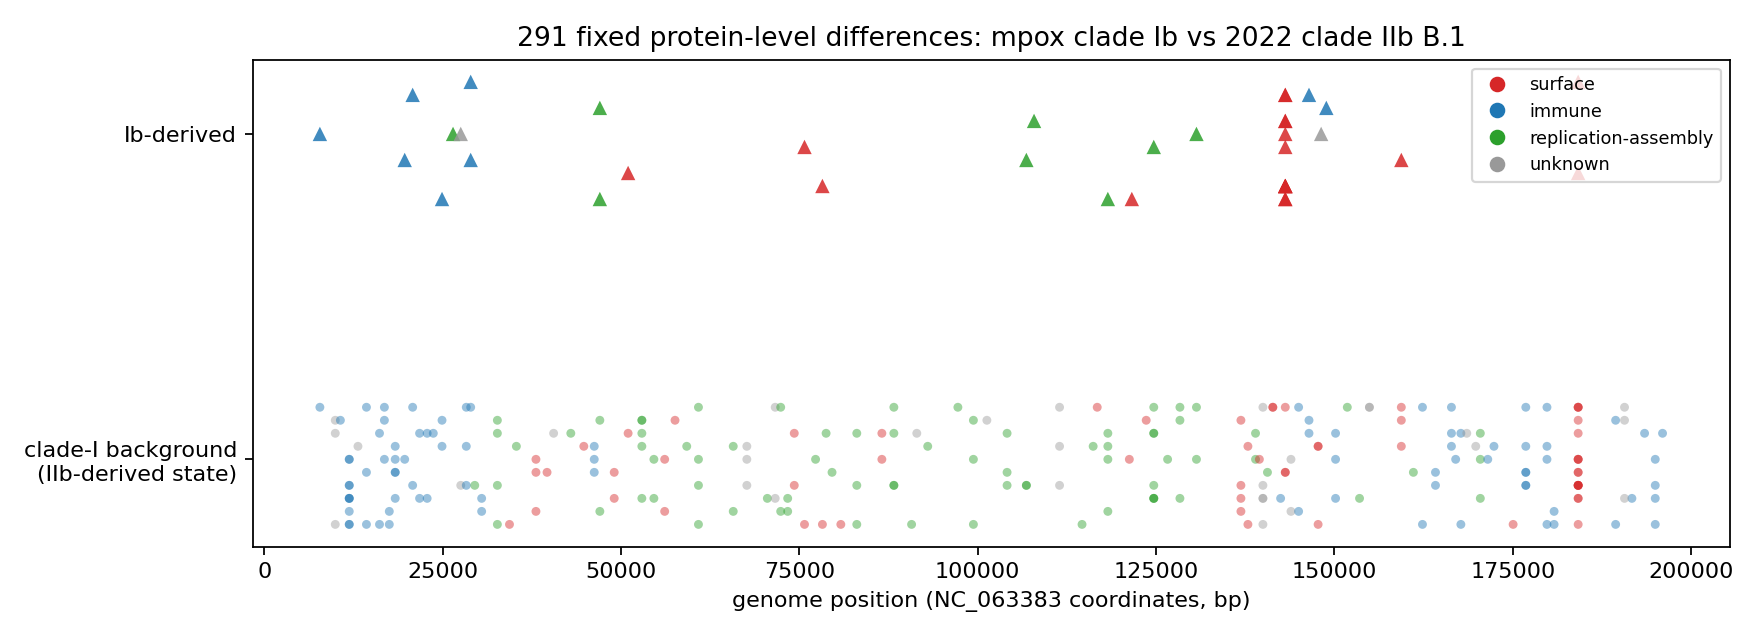
\includegraphics[width=\textwidth]{fig1.png}
\caption{Genome distribution of 291 fixed differences (Ib-derived highlighted).}\end{figure}
\begin{figure}[h]\centering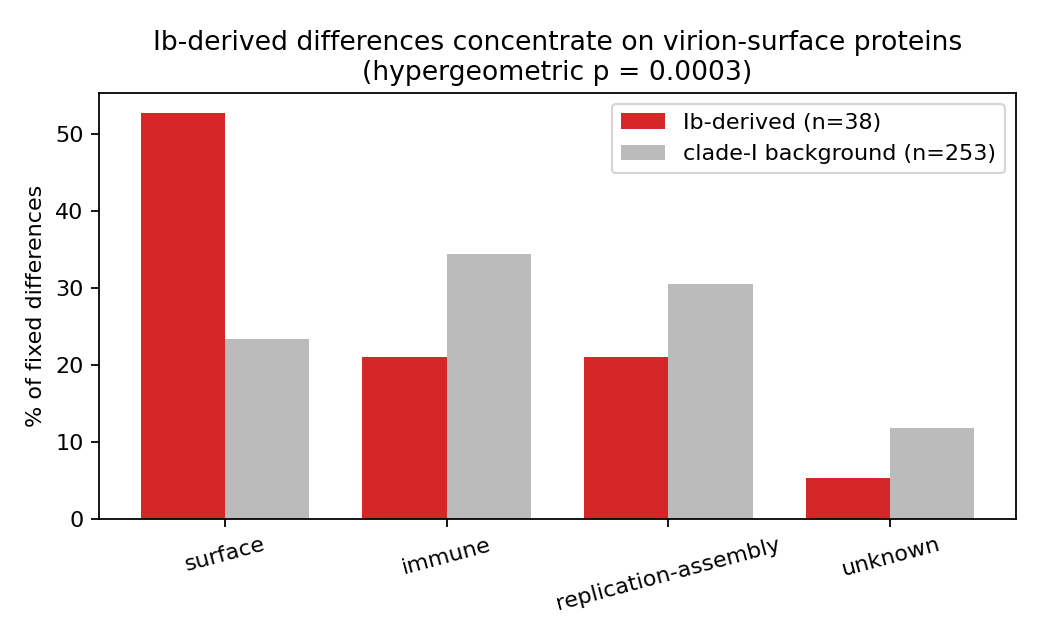
\includegraphics[width=0.75\textwidth]{fig2.png}
\caption{Protein-class composition of Ib-derived vs background fixed differences.}\end{figure}
\begin{figure}[h]\centering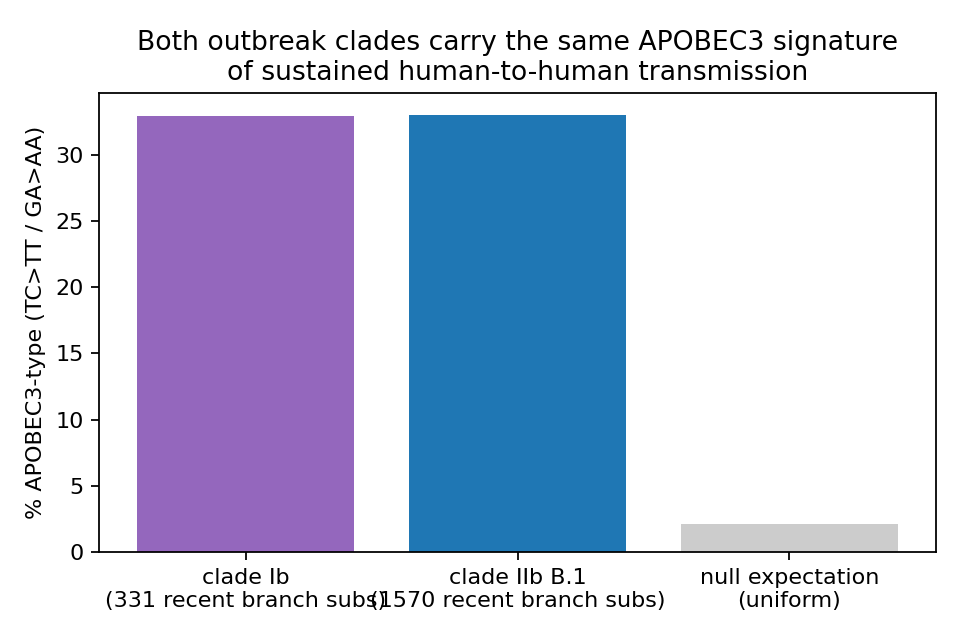
\includegraphics[width=0.7\textwidth]{fig3.png}
\caption{APOBEC3-type substitution fractions in recent evolution of both clades vs null.}\end{figure}
\begin{figure}[h]\centering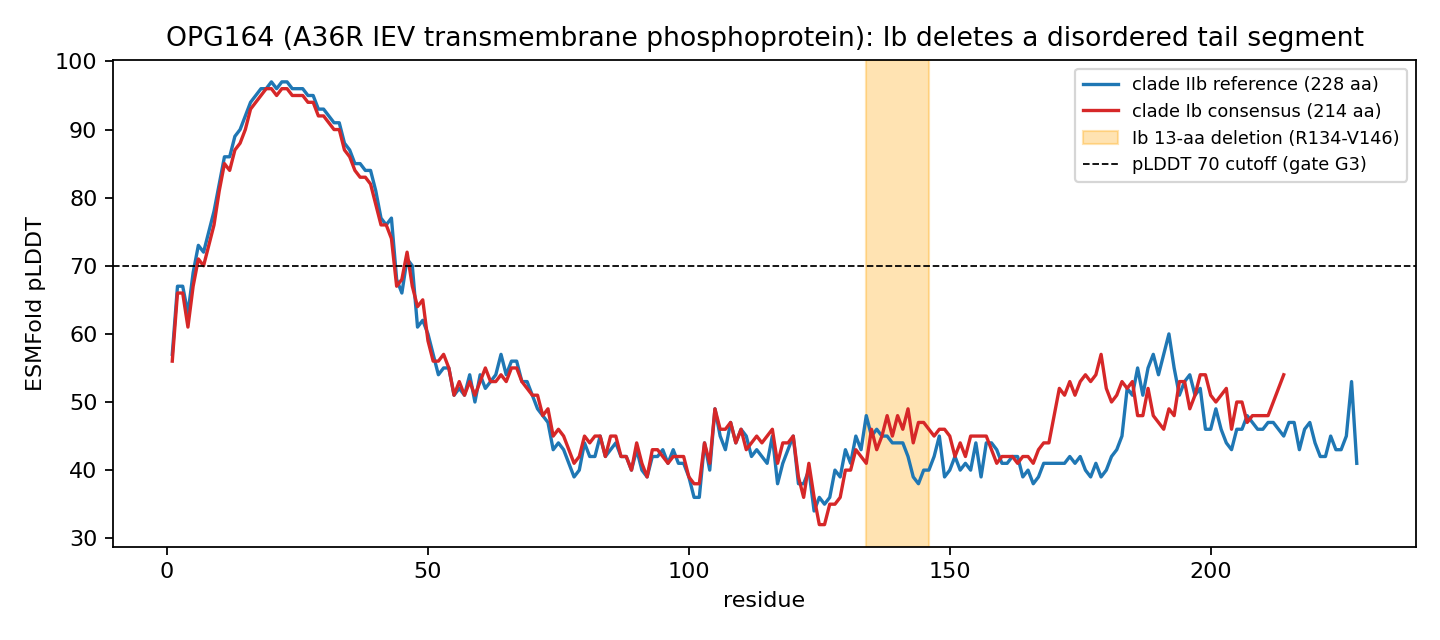
\includegraphics[width=0.9\textwidth]{fig4.png}
\caption{OPG164/A36R ESMFold pLDDT profiles; the Ib 13-aa deletion spans a disordered tail
segment.}\end{figure}

\clearpage
\section*{Table 1. All 38 Ib-derived fixed differences}
\begin{longtable}{lllll}
\hline Gene & Change & Protein & Class & Ib freq \\ \hline \endhead
OPG019 & G112C & EGF-like domain protein & immune & 0.9947 \\
OPG034 & P184H & Bcl-2-like protein & immune & 0.9972 \\
OPG036 & V17I & Bcl-2-like protein & immune & 1.0 \\
OPG040 & M160I & Serpin & immune & 1.0 \\
OPG042 & T159I & Phospholipase-D-like protein & replication-assembly & 1.0 \\
OPG043 & N68S & Putative monoglyceride lipase & unknown & 0.9973 \\
OPG045 & V16- & Caspase-9 inhibitor & immune & 0.9833 \\
OPG045 & H17- & Caspase-9 inhibitor & immune & 0.9804 \\
OPG066 & K140N & DNA-directed RNA polymerase 30 kDa pol & replication-assembly & 1.0 \\
OPG066 & L222I & DNA-directed RNA polymerase 30 kDa pol & replication-assembly & 1.0 \\
OPG070 & Y12H & Membrane protein E8 & surface & 1.0 \\
OPG096 & L75P & Crescent membrane and immature virion  & surface & 0.9973 \\
OPG100 & R134H & IMV membrane protein J1 & surface & 1.0 \\
OPG125 & T493M & Rifampicin resistance protein & replication-assembly & 1.0 \\
OPG126 & A26S & Late transcription factor VLTF-2 (2) & replication-assembly & 0.9973 \\
OPG136 & M740I & Virion core protein P4a & replication-assembly & 0.9973 \\
OPG140 & P39H & IMV membrane protein A14 & surface & 1.0 \\
OPG145 & P76Q & DNA helicase & replication-assembly & 1.0 \\
OPG151 & R273Q & DNA-dependent RNA polymerase subunit r & replication-assembly & 1.0 \\
OPG164 & R134- & IEV transmembrane phosphoprotein & surface & 0.9966 \\
OPG164 & N135- & IEV transmembrane phosphoprotein & surface & 1.0 \\
OPG164 & E136- & IEV transmembrane phosphoprotein & surface & 1.0 \\
OPG164 & Q137- & IEV transmembrane phosphoprotein & surface & 0.9967 \\
OPG164 & T138- & IEV transmembrane phosphoprotein & surface & 0.9967 \\
OPG164 & I139- & IEV transmembrane phosphoprotein & surface & 0.9967 \\
OPG164 & Y140- & IEV transmembrane phosphoprotein & surface & 0.9967 \\
OPG164 & Q141- & IEV transmembrane phosphoprotein & surface & 0.9935 \\
OPG164 & N142- & IEV transmembrane phosphoprotein & surface & 0.9935 \\
OPG164 & T143- & IEV transmembrane phosphoprotein & surface & 0.9935 \\
OPG164 & T144- & IEV transmembrane phosphoprotein & surface & 0.9935 \\
OPG164 & V145- & IEV transmembrane phosphoprotein & surface & 0.9935 \\
OPG164 & V146- & IEV transmembrane phosphoprotein & surface & 0.9561 \\
OPG170 & V96I & Chemokine binding protein & immune & 1.0 \\
OPG173 & N21S & MPXVgp154 & unknown & 1.0 \\
OPG174 & R315C & Hydroxysteroid dehydrogenase & immune & 1.0 \\
OPG185 & T239I & Hemagglutinin & surface & 0.997 \\
OPG210 & A475V & B22R family protein & surface & 1.0 \\
OPG210 & E1057D & B22R family protein & surface & 1.0 \\
\hline
\end{longtable}

\clearpage
\appendix
\section*{Appendix Table A1. All 291 fixed differences (Ib vs IIb B.1)}
\begin{longtable}{lllll}
\hline Gene & Change & Protein & Category & Class \\ \hline \endhead
OPG001 & S105L & Chemokine binding protein & IIb-derived & immune \\
OPG002 & S54F & Crm-B secreted TNF-alpha-recepto & IIb-derived & immune \\
OPG002 & A121A & Crm-B secreted TNF-alpha-recepto & IIb-derived & immune \\
OPG002 & V172V & Crm-B secreted TNF-alpha-recepto & IIb-derived & immune \\
OPG002 & N313N & Crm-B secreted TNF-alpha-recepto & IIb-derived & immune \\
OPG003 & D264N & Ankyrin repeat protein (25) & IIb-derived & immune \\
OPG015 & L136L & Ankyrin repeat protein (39) & IIb-derived & immune \\
OPG019 & G112C & EGF-like domain protein & Ib-derived & immune \\
OPG019 & M124M & EGF-like domain protein & IIb-derived & immune \\
OPG021 & V38V & Zinc finger-like protein (2) & IIb-derived & unknown \\
OPG021 & S219S & Zinc finger-like protein (2) & IIb-derived & unknown \\
OPG021 & K230K & Zinc finger-like protein (2) & IIb-derived & unknown \\
OPG022 & G73G & Interleukin-18-binding protein & IIb-derived & immune \\
OPG023 & M109M & Ankyrin repeat protein (2) & IIb-derived & immune \\
OPG023 & V174V & Ankyrin repeat protein (2) & IIb-derived & immune \\
OPG023 & A193A & Ankyrin repeat protein (2) & IIb-derived & immune \\
OPG023 & S258S & Ankyrin repeat protein (2) & IIb-derived & immune \\
OPG023 & Y300Y & Ankyrin repeat protein (2) & IIb-derived & immune \\
OPG023 & C304C & Ankyrin repeat protein (2) & IIb-derived & immune \\
OPG023 & V426V & Ankyrin repeat protein (2) & IIb-derived & immune \\
OPG023 & T488T & Ankyrin repeat protein (2) & IIb-derived & immune \\
OPG023 & L602L & Ankyrin repeat protein (2) & IIb-derived & immune \\
OPG023 & K637K & Ankyrin repeat protein (2) & IIb-derived & immune \\
OPG024 & S32S & retroviral pseudoprotease-like p & IIb-derived & unknown \\
OPG025 & E393E & Ankyrin repeat protein (14) & IIb-derived & immune \\
OPG025 & A423D & Ankyrin repeat protein (14) & IIb-derived & immune \\
OPG025 & I425I & Ankyrin repeat protein (14) & IIb-derived & immune \\
OPG027 & I47I & Host range protein & IIb-derived & immune \\
OPG027 & V126V & Host range protein & IIb-derived & immune \\
OPG029 & C146C & Bcl-2-like protein & IIb-derived & immune \\
OPG029 & D153D & Bcl-2-like protein & IIb-derived & immune \\
OPG029 & D154D & Bcl-2-like protein & IIb-derived & immune \\
OPG030 & N12N & Kelch-like protein (1) & IIb-derived & immune \\
OPG030 & S113S & Kelch-like protein (1) & IIb-derived & immune \\
OPG031 & T80T & C4L/C10L-like family protein & IIb-derived & immune \\
OPG031 & D117D & C4L/C10L-like family protein & IIb-derived & immune \\
OPG031 & C241C & C4L/C10L-like family protein & IIb-derived & immune \\
OPG031 & G258G & C4L/C10L-like family protein & IIb-derived & immune \\
OPG031 & M271M & C4L/C10L-like family protein & IIb-derived & immune \\
OPG034 & P184H & Bcl-2-like protein & Ib-derived & immune \\
OPG034 & L205L & Bcl-2-like protein & IIb-derived & immune \\
OPG036 & S11S & Bcl-2-like protein & IIb-derived & immune \\
OPG036 & V17I & Bcl-2-like protein & Ib-derived & immune \\
OPG036 & D25D & Bcl-2-like protein & IIb-derived & immune \\
OPG037 & C144C & Ankyrin-like protein (1) & IIb-derived & immune \\
OPG037 & C415C & Ankyrin-like protein (1) & IIb-derived & immune \\
OPG038 & H27H & NFkB inhibitor & IIb-derived & immune \\
OPG038 & V78V & NFkB inhibitor & IIb-derived & immune \\
OPG039 & C279C & Ankyrin-like protein (3) & IIb-derived & immune \\
OPG040 & M160I & Serpin & Ib-derived & immune \\
OPG040 & P254P & Serpin & IIb-derived & immune \\
OPG040 & Y374Y & Serpin & IIb-derived & immune \\
OPG042 & T159I & Phospholipase-D-like protein & Ib-derived & replication-assembly \\
OPG043 & T3T & Putative monoglyceride lipase & IIb-derived & unknown \\
OPG043 & N68S & Putative monoglyceride lipase & Ib-derived & unknown \\
OPG044 & V63V & Bcl-2-like protein & IIb-derived & immune \\
OPG044 & T109T & Bcl-2-like protein & IIb-derived & immune \\
OPG044 & M148M & Bcl-2-like protein & IIb-derived & immune \\
OPG045 & V16- & Caspase-9 inhibitor & Ib-derived & immune \\
OPG045 & H17- & Caspase-9 inhibitor & Ib-derived & immune \\
OPG045 & A185A & Caspase-9 inhibitor & IIb-derived & immune \\
OPG046 & S95S & dUTPase & IIb-derived & replication-assembly \\
OPG047 & R48C & Kelch-like protein (2) & IIb-derived & immune \\
OPG047 & I232I & Kelch-like protein (2) & IIb-derived & immune \\
OPG049 & E17E & Telomere-binding protein I6 (1) & IIb-derived & replication-assembly \\
OPG049 & M37M & Telomere-binding protein I6 (1) & IIb-derived & replication-assembly \\
OPG049 & T263T & Telomere-binding protein I6 (1) & IIb-derived & replication-assembly \\
OPG049 & R314R & Telomere-binding protein I6 (1) & IIb-derived & replication-assembly \\
OPG053 & P78S & IMV membrane protein L1R & IIb-derived & surface \\
OPG054 & R438R & Serine/threonine-protein kinase & IIb-derived & replication-assembly \\
OPG056 & E125K & EEV maturation protein & IIb-derived & surface \\
OPG056 & V323V & EEV maturation protein & IIb-derived & surface \\
OPG056 & C622C & EEV maturation protein & IIb-derived & surface \\
OPG057 & E353K & Palmytilated EEV membrane protei & IIb-derived & surface \\
OPG059 & I26I & Cytochrome C oxidase & IIb-derived & unknown \\
OPG063 & V307V & Poly(A) polymerase catalytic sub & IIb-derived & replication-assembly \\
OPG064 & A88A & Iev morphogenesis protein & IIb-derived & surface \\
OPG065 & A17A & Double-stranded RNA binding prot & IIb-derived & immune \\
OPG065 & N23N & Double-stranded RNA binding prot & IIb-derived & immune \\
OPG065 & H61H & Double-stranded RNA binding prot & IIb-derived & immune \\
OPG066 & K83K & DNA-directed RNA polymerase 30 k & IIb-derived & replication-assembly \\
OPG066 & H97H & DNA-directed RNA polymerase 30 k & IIb-derived & replication-assembly \\
OPG066 & K140N & DNA-directed RNA polymerase 30 k & Ib-derived & replication-assembly \\
OPG066 & L222I & DNA-directed RNA polymerase 30 k & Ib-derived & replication-assembly \\
OPG068 & P251P & IMV membrane protein E6 & IIb-derived & surface \\
OPG068 & D341D & IMV membrane protein E6 & IIb-derived & surface \\
OPG070 & Y12H & Membrane protein E8 & Ib-derived & surface \\
OPG070 & H205H & Membrane protein E8 & IIb-derived & surface \\
OPG071 & L108F & DNA polymerase (2) & IIb-derived & replication-assembly \\
OPG071 & L411L & DNA polymerase (2) & IIb-derived & replication-assembly \\
OPG071 & I428I & DNA polymerase (2) & IIb-derived & replication-assembly \\
OPG071 & A484A & DNA polymerase (2) & IIb-derived & replication-assembly \\
OPG071 & I501I & DNA polymerase (2) & IIb-derived & replication-assembly \\
OPG072 & V10V & Sulfhydryl oxidase & IIb-derived & replication-assembly \\
OPG072 & D56N & Sulfhydryl oxidase & IIb-derived & replication-assembly \\
OPG074 & N199N & Iev morphogenesis protein & IIb-derived & surface \\
OPG074 & I441I & Iev morphogenesis protein & IIb-derived & surface \\
OPG076 & S20S & MV membrane EFC component & IIb-derived & surface \\
OPG079 & C45C & DNA-binding phosphoprotein (2) & IIb-derived & replication-assembly \\
OPG080 & D321D & Ribonucleoside-diphosphate reduc & IIb-derived & replication-assembly \\
OPG080 & C382C & Ribonucleoside-diphosphate reduc & IIb-derived & replication-assembly \\
OPG080 & L521L & Ribonucleoside-diphosphate reduc & IIb-derived & replication-assembly \\
OPG080 & P582P & Ribonucleoside-diphosphate reduc & IIb-derived & replication-assembly \\
OPG084 & S211S & RNA helicase NPH-II (2) & IIb-derived & replication-assembly \\
OPG084 & Q620Q & RNA helicase NPH-II (2) & IIb-derived & replication-assembly \\
OPG085 & S79S & Metalloendopeptidase & IIb-derived & unknown \\
OPG085 & T328T & Metalloendopeptidase & IIb-derived & unknown \\
OPG085 & F591F & Metalloendopeptidase & IIb-derived & unknown \\
OPG089 & D303D & FEN1-like nuclease & IIb-derived & replication-assembly \\
OPG091 & V62V & Nlpc/p60 superfamily protein & IIb-derived & unknown \\
OPG091 & S73S & Nlpc/p60 superfamily protein & IIb-derived & unknown \\
OPG092 & D196N & Assembly protein G7 & IIb-derived & replication-assembly \\
OPG092 & I244I & Assembly protein G7 & IIb-derived & replication-assembly \\
OPG093 & S30L & Late transcription factor VLTF-1 & IIb-derived & replication-assembly \\
OPG093 & D88N & Late transcription factor VLTF-1 & IIb-derived & replication-assembly \\
OPG094 & M142I & Myristylated protein & IIb-derived & surface \\
OPG094 & R175R & Myristylated protein & IIb-derived & surface \\
OPG096 & I68I & Crescent membrane and immature v & IIb-derived & surface \\
OPG096 & L75P & Crescent membrane and immature v & Ib-derived & surface \\
OPG098 & E162K & Nucleic acid binding protein VP8 & IIb-derived & replication-assembly \\
OPG100 & R134H & IMV membrane protein J1 & Ib-derived & surface \\
OPG100 & K152K & IMV membrane protein J1 & IIb-derived & surface \\
OPG101 & T153T & Thymidine kinase & IIb-derived & replication-assembly \\
OPG102 & I249I & Cap-specific mRNA & IIb-derived & replication-assembly \\
OPG104 & T12T & Myristylated protein & IIb-derived & surface \\
OPG105 & V113V & DNA-dependent RNA polymerase sub & IIb-derived & replication-assembly \\
OPG105 & S734L & DNA-dependent RNA polymerase sub & IIb-derived & replication-assembly \\
OPG105 & I1070I & DNA-dependent RNA polymerase sub & IIb-derived & replication-assembly \\
OPG108 & V4V & IMV heparin binding surface prot & IIb-derived & surface \\
OPG108 & T111T & IMV heparin binding surface prot & IIb-derived & surface \\
OPG109 & R364R & RNA polymerase-associated transc & IIb-derived & replication-assembly \\
OPG109 & A622A & RNA polymerase-associated transc & IIb-derived & replication-assembly \\
OPG109 & A630A & RNA polymerase-associated transc & IIb-derived & replication-assembly \\
OPG109 & H740Y & RNA polymerase-associated transc & IIb-derived & replication-assembly \\
OPG111 & I77I & DNA topoisomerase type I & IIb-derived & replication-assembly \\
OPG112 & H34H & Late protein H7 & IIb-derived & unknown \\
OPG113 & V537V & mRNA capping enzyme large subuni & IIb-derived & replication-assembly \\
OPG117 & D454D & NTPase (1) & IIb-derived & replication-assembly \\
OPG118 & K256K & Early transcription factor 70 kD & IIb-derived & replication-assembly \\
OPG118 & N413N & Early transcription factor 70 kD & IIb-derived & replication-assembly \\
OPG118 & V462V & Early transcription factor 70 kD & IIb-derived & replication-assembly \\
OPG120 & A19A & Carbonic anhydrase & IIb-derived & unknown \\
OPG123 & I172I & Nucleoside triphosphatase I & IIb-derived & replication-assembly \\
OPG123 & A313A & Nucleoside triphosphatase I & IIb-derived & replication-assembly \\
OPG123 & C436C & Nucleoside triphosphatase I & IIb-derived & replication-assembly \\
OPG125 & E111E & Rifampicin resistance protein & IIb-derived & replication-assembly \\
OPG125 & T493M & Rifampicin resistance protein & Ib-derived & replication-assembly \\
OPG125 & I514I & Rifampicin resistance protein & IIb-derived & replication-assembly \\
OPG126 & A26S & Late transcription factor VLTF-2 & Ib-derived & replication-assembly \\
OPG130 & T63T & A5L protein-like & IIb-derived & unknown \\
OPG130 & T122T & A5L protein-like & IIb-derived & unknown \\
OPG130 & L270L & A5L protein-like & IIb-derived & unknown \\
OPG133 & F594F & Early transcription factor 82 kD & IIb-derived & replication-assembly \\
OPG134 & E226E & Intermediate transcription facto & IIb-derived & replication-assembly \\
OPG135 & V90V & IMV membrane protein A9 & IIb-derived & surface \\
OPG136 & D98N & Virion core protein P4a & IIb-derived & replication-assembly \\
OPG136 & A229A & Virion core protein P4a & IIb-derived & replication-assembly \\
OPG136 & D267D & Virion core protein P4a & IIb-derived & replication-assembly \\
OPG136 & F283F & Virion core protein P4a & IIb-derived & replication-assembly \\
OPG136 & M740I & Virion core protein P4a & Ib-derived & replication-assembly \\
OPG139 & A17T & IMV membrane protein A13L & IIb-derived & surface \\
OPG140 & P39H & IMV membrane protein A14 & Ib-derived & surface \\
OPG144 & T184T & IMV membrane protein P21 & IIb-derived & surface \\
OPG145 & E62K & DNA helicase & IIb-derived & replication-assembly \\
OPG145 & P76Q & DNA helicase & Ib-derived & replication-assembly \\
OPG145 & R243Q & DNA helicase & IIb-derived & replication-assembly \\
OPG145 & I249I & DNA helicase & IIb-derived & replication-assembly \\
OPG145 & I264I & DNA helicase & IIb-derived & replication-assembly \\
OPG145 & A348A & DNA helicase & IIb-derived & replication-assembly \\
OPG145 & E435K & DNA helicase & IIb-derived & replication-assembly \\
OPG145 & Q463Q & DNA helicase & IIb-derived & replication-assembly \\
OPG148 & I313I & DNA polymerase processivity fact & IIb-derived & replication-assembly \\
OPG150 & N100N & Intermediate transcription facto & IIb-derived & replication-assembly \\
OPG150 & D256D & Intermediate transcription facto & IIb-derived & replication-assembly \\
OPG150 & S307L & Intermediate transcription facto & IIb-derived & replication-assembly \\
OPG151 & D6D & DNA-dependent RNA polymerase sub & IIb-derived & replication-assembly \\
OPG151 & R273Q & DNA-dependent RNA polymerase sub & Ib-derived & replication-assembly \\
OPG151 & N282N & DNA-dependent RNA polymerase sub & IIb-derived & replication-assembly \\
OPG153 & M14M & Orthopoxvirus A26L/A30L protein & IIb-derived & surface \\
OPG153 & I355I & Orthopoxvirus A26L/A30L protein & IIb-derived & surface \\
OPG153 & Y358Y & Orthopoxvirus A26L/A30L protein & IIb-derived & surface \\
OPG153 & Q493Q & Orthopoxvirus A26L/A30L protein & IIb-derived & surface \\
OPG154 & R74R & IMV surface fusion protein & IIb-derived & surface \\
OPG154 & H107H & IMV surface fusion protein & IIb-derived & surface \\
OPG156 & Y42Y & DNA-directed RNA polymerase 35 k & IIb-derived & replication-assembly \\
OPG156 & T222T & DNA-directed RNA polymerase 35 k & IIb-derived & replication-assembly \\
OPG157 & M24M & IMV membrane protein A30 & IIb-derived & surface \\
OPG159 & T2T & CPXV166 protein & IIb-derived & unknown \\
OPG159 & L36L & CPXV166 protein & IIb-derived & unknown \\
OPG159 & N124- & CPXV166 protein & outgroup-uncertain & unknown \\
OPG159 & Y125- & CPXV166 protein & outgroup-uncertain & unknown \\
OPG159 & N126- & CPXV166 protein & outgroup-uncertain & unknown \\
OPG160 & P2P & ATPase A32 & IIb-derived & replication-assembly \\
OPG161 & K67K & EEV glycoprotein (1) & IIb-derived & surface \\
OPG161 & V88V & EEV glycoprotein (1) & IIb-derived & surface \\
OPG163 & V46V & MHC class II antigen presentatio & IIb-derived & immune \\
OPG164 & I111I & IEV transmembrane phosphoprotein & IIb-derived & surface \\
OPG164 & R134- & IEV transmembrane phosphoprotein & Ib-derived & surface \\
OPG164 & N135- & IEV transmembrane phosphoprotein & Ib-derived & surface \\
OPG164 & E136- & IEV transmembrane phosphoprotein & Ib-derived & surface \\
OPG164 & Q137- & IEV transmembrane phosphoprotein & Ib-derived & surface \\
OPG164 & T138- & IEV transmembrane phosphoprotein & Ib-derived & surface \\
OPG164 & I139- & IEV transmembrane phosphoprotein & Ib-derived & surface \\
OPG164 & Y140- & IEV transmembrane phosphoprotein & Ib-derived & surface \\
OPG164 & Q141- & IEV transmembrane phosphoprotein & Ib-derived & surface \\
OPG164 & N142- & IEV transmembrane phosphoprotein & Ib-derived & surface \\
OPG164 & T143- & IEV transmembrane phosphoprotein & Ib-derived & surface \\
OPG164 & T144- & IEV transmembrane phosphoprotein & Ib-derived & surface \\
OPG164 & V145- & IEV transmembrane phosphoprotein & Ib-derived & surface \\
OPG164 & V146- & IEV transmembrane phosphoprotein & Ib-derived & surface \\
OPG164 & Y217Y & IEV transmembrane phosphoprotein & IIb-derived & surface \\
OPG164 & V228V & IEV transmembrane phosphoprotein & IIb-derived & surface \\
OPG165 & D106D & CPXV173 protein & IIb-derived & unknown \\
OPG165 & S161S & CPXV173 protein & IIb-derived & unknown \\
OPG167 & Y107Y & CD47-like protein & IIb-derived & immune \\
OPG167 & I112I & CD47-like protein & IIb-derived & immune \\
OPG170 & G31G & Chemokine binding protein & IIb-derived & immune \\
OPG170 & V96I & Chemokine binding protein & Ib-derived & immune \\
OPG170 & M111M & Chemokine binding protein & IIb-derived & immune \\
OPG172 & A125A & Type-I membrane glycoprotein & IIb-derived & surface \\
OPG172 & M145M & Type-I membrane glycoprotein & IIb-derived & surface \\
OPG172 & Y160Y & Type-I membrane glycoprotein & IIb-derived & surface \\
OPG173 & N21S & MPXVgp154 & Ib-derived & unknown \\
OPG174 & R315C & Hydroxysteroid dehydrogenase & Ib-derived & immune \\
OPG176 & D24D & Bcl-2-like protein & IIb-derived & immune \\
OPG176 & H221Y & Bcl-2-like protein & IIb-derived & immune \\
OPG176 & L227L & Bcl-2-like protein & IIb-derived & immune \\
OPG178 & I139I & Thymidylate kinase & IIb-derived & replication-assembly \\
OPG180 & L555L & DNA ligase (2) & IIb-derived & replication-assembly \\
OPG181 & L85L & M137R & IIb-derived & unknown \\
OPG181 & S127S & M137R & IIb-derived & unknown \\
OPG185 & T167T & Hemagglutinin & IIb-derived & surface \\
OPG185 & D177D & Hemagglutinin & IIb-derived & surface \\
OPG185 & I205I & Hemagglutinin & IIb-derived & surface \\
OPG185 & T239I & Hemagglutinin & Ib-derived & surface \\
OPG187 & K300K & Ser/thr kinase & IIb-derived & replication-assembly \\
OPG188 & V265V & Schlafen (1) & IIb-derived & immune \\
OPG188 & S419S & Schlafen (1) & IIb-derived & immune \\
OPG189 & K185K & Ankyrin repeat protein (25) & IIb-derived & immune \\
OPG189 & C506C & Ankyrin repeat protein (25) & IIb-derived & immune \\
OPG191 & P50P & Ankyrin-like protein (46) & IIb-derived & immune \\
OPG191 & F80F & Ankyrin-like protein (46) & IIb-derived & immune \\
OPG191 & F166F & Ankyrin-like protein (46) & IIb-derived & immune \\
OPG192 & G100G & Virulence protein & IIb-derived & immune \\
OPG193 & I108I & Soluble interferon-gamma recepto & IIb-derived & immune \\
OPG193 & L263F & Soluble interferon-gamma recepto & IIb-derived & immune \\
OPG195 & C120C & Intracellular viral protein & IIb-derived & unknown \\
OPG197 & M1M & CPXV205 protein & IIb-derived & unknown \\
OPG198 & N71N & Ser/thr kinase & IIb-derived & replication-assembly \\
OPG198 & I100I & Ser/thr kinase & IIb-derived & replication-assembly \\
OPG198 & Q133Q & Ser/thr kinase & IIb-derived & replication-assembly \\
OPG199 & K230K & Serpin & IIb-derived & immune \\
OPG200 & E134E & Bcl-2-like protein & IIb-derived & immune \\
OPG204 & N178N & IFN-alpha/beta-receptor-like sec & IIb-derived & surface \\
OPG205 & W169W & Ankyrin repeat protein (44) & IIb-derived & immune \\
OPG205 & C349C & Ankyrin repeat protein (44) & IIb-derived & immune \\
OPG205 & G354G & Ankyrin repeat protein (44) & IIb-derived & immune \\
OPG205 & V621V & Ankyrin repeat protein (44) & IIb-derived & immune \\
OPG205 & V690V & Ankyrin repeat protein (44) & IIb-derived & immune \\
OPG205 & R733R & Ankyrin repeat protein (44) & IIb-derived & immune \\
OPG208 & A34A & Serpin & IIb-derived & immune \\
OPG208 & I142I & Serpin & IIb-derived & immune \\
OPG208 & T300T & Serpin & IIb-derived & immune \\
OPG208 & V311V & Serpin & IIb-derived & immune \\
OPG209 & I11I & Virulence protein & IIb-derived & immune \\
OPG209 & L21L & Virulence protein & IIb-derived & immune \\
OPG210 & F3F & B22R family protein & IIb-derived & surface \\
OPG210 & A98A & B22R family protein & IIb-derived & surface \\
OPG210 & V173V & B22R family protein & IIb-derived & surface \\
OPG210 & D209N & B22R family protein & IIb-derived & surface \\
OPG210 & K331K & B22R family protein & IIb-derived & surface \\
OPG210 & N334N & B22R family protein & IIb-derived & surface \\
OPG210 & H363H & B22R family protein & IIb-derived & surface \\
OPG210 & D379D & B22R family protein & IIb-derived & surface \\
OPG210 & A475V & B22R family protein & Ib-derived & surface \\
OPG210 & V515V & B22R family protein & IIb-derived & surface \\
OPG210 & P722S & B22R family protein & IIb-derived & surface \\
OPG210 & L734L & B22R family protein & IIb-derived & surface \\
OPG210 & S781S & B22R family protein & IIb-derived & surface \\
OPG210 & V788V & B22R family protein & IIb-derived & surface \\
OPG210 & T928T & B22R family protein & IIb-derived & surface \\
OPG210 & E1057D & B22R family protein & Ib-derived & surface \\
OPG210 & A1305A & B22R family protein & IIb-derived & surface \\
OPG210 & L1704L & B22R family protein & IIb-derived & surface \\
OPG210 & D1717D & B22R family protein & IIb-derived & surface \\
OPG210 & M1741I & B22R family protein & IIb-derived & surface \\
OPG005 & S3S & Bcl-2-like protein & IIb-derived & immune \\
OPG005 & N74N & Bcl-2-like protein & IIb-derived & immune \\
OPG016 & S63S & Brix domain protein & IIb-derived & unknown \\
OPG016 & E80E & Brix domain protein & IIb-derived & unknown \\
OPG016 & D121D & Brix domain protein & IIb-derived & unknown \\
\hline
\end{longtable}
\end{document}
